% --- SLIDE: Learning Outcomes ---
\begin{frame}{Learning Outcomes}
\textbf{By the end of this session, you will be able to:}

\vspace{1em}
\begin{itemize}\setlength\itemsep{1em}
    \item Differentiate between Supervised and Unsupervised Learning paradigms.
    \item Understand K-Means clustering, and how it could be applied to discover hidden groups in data.
    \item Analyze high-dimensional data using PCA and t-SNE for visualization and compression.
    \item Understand how Autoencoders utilize neural networks for tasks like denoising, generation, and anomaly detection.
\end{itemize}

\end{frame}

\begin{frame}{Table of Contents}
    \tableofcontents
\end{frame}


% =========================
% 7. Unsupervised Learning
% =========================
\section{Unsupervised Learning}

% --- SLIDE: What is Unsupervised Learning? ---
\begin{frame}{What is Unsupervised Learning?}
\textbf{So far:} We've been doing \textbf{Supervised Learning}, learning from labeled data $(x, y)$.

\vspace{1em}
\begin{columns}[c]
\begin{column}{0.50\textwidth}
\begin{tcolorbox}[colback=blue!5, colframe=blue!50, title=\textbf{Supervised Learning}]
\textbf{Data:} $(x, y)$ pairs
\begin{itemize}
\item $x$: input (features)
\item $y$: label (target)
\end{itemize}
\vspace{0.3em}
\textbf{Goal:} Learn $f(x) \approx y$

\textbf{Examples:}
\begin{itemize}
\item Image classification
\item House price prediction
\end{itemize}
\end{tcolorbox}
\end{column}

\begin{column}{0.50\textwidth}
\begin{tcolorbox}[colback=green!5, colframe=green!50!black, title=\textbf{Unsupervised Learning}]
\textbf{Data:} Only $x$ (no labels!)
\begin{itemize}
\item Just raw data
\item No target to predict
\end{itemize}
\vspace{0.3em}
\textbf{Goal:} Find hidden patterns or structure

\textbf{Examples:}
\begin{itemize}
\item Customer segmentation
\item Data compression
\end{itemize}
\end{tcolorbox}
\end{column}
\end{columns}

\vspace{1em}
\centering
\textbf{Key difference:} No labels $\rightarrow$ algorithm must discover structure on its own!
\end{frame}

% --- SLIDE: Why Unsupervised Learning? ---
\begin{frame}{Why Unsupervised Learning?}
\textbf{Labels are expensive!}

\vspace{0.5em}
\begin{itemize}
\item Labeling data requires human effort, time, and expertise
\item Most real-world data is unlabeled
\item Sometimes we don't even know what labels to look for
\end{itemize}

\vspace{1em}
\begin{tcolorbox}[colback=yellow!8, colframe=orange!60, title=\textbf{The Big Idea}]
Can we learn useful things from data \textbf{without} labels? \\
Yes! Unsupervised learning finds hidden patterns, structure, and representations.
\end{tcolorbox}

\end{frame}

% --- SLIDE: Tasks in Unsupervised Learning ---
\begin{frame}{Common Unsupervised Learning Tasks}
\textbf{What can we do without labels?}

% \vspace{0.8em}
\begin{columns}[t]
\begin{column}{0.52\textwidth}
\begin{tcolorbox}[colback=blue!5, colframe=blue!50, height=2.7cm]
\textbf{1. Clustering}

Group similar data points together

\textbf{Example:} Customer segmentation, document group
\end{tcolorbox}

\vspace{0.5em}

\begin{tcolorbox}[colback=red!5, colframe=red!50, height=2.7cm]
\textbf{2. Dimensionality Reduction}

Compress high-dimensional data to lower dimensions

\textbf{Example:} Visualization, feature extraction
\end{tcolorbox}
\end{column}

\begin{column}{0.50\textwidth}
\begin{tcolorbox}[colback=orange!5, colframe=orange!50, height=2.7cm]
\textbf{3. Anomaly Detection}

Identify unusual or outlier data points

\textbf{Example:} Fraud detection, quality control
\end{tcolorbox}

\vspace{0.5em}

\begin{tcolorbox}[colback=purple!5, colframe=purple!50, height=2.7cm]
\textbf{4. Generation}

Learn to create new, realistic data samples

\textbf{Example:} Image synthesis, data augmentation
\end{tcolorbox}
\end{column}
\end{columns}

\vspace{0.5em}
\centering
\small \textit{We'll explore four powerful algorithms that tackle these tasks.}
\end{frame}

% =========================
% K-Means Clustering - IMPROVED VERSION
% =========================

% --- SLIDE 1: What is Clustering? ---
% \begin{frame}{What is Clustering?}

% \textbf{Goal:} Group similar data points together without labels

% \vspace{0.5em}
% \begin{columns}[c]
% \begin{column}{0.48\textwidth}
% \textbf{Supervised vs Unsupervised}

% \vspace{0.5em}
% \begin{tcolorbox}[colback=blue!5, colframe=blue!50]
% \textbf{Supervised}\\
% \small
% Data: $(x, y)$ with labels\\
% Goal: Learn $f(x) \rightarrow y$\\
% Example: Cat vs Dog classifier
% \end{tcolorbox}

% \vspace{0.3em}
% \begin{tcolorbox}[colback=green!5, colframe=green!50!black]
% \textbf{Unsupervised (Clustering)}\\
% \small
% Data: $x$ only, no labels\\
% Goal: Find natural groups\\
% Example: Customer segments
% \end{tcolorbox}
% \end{column}

% \begin{column}{0.48\textwidth}
% \centering
% \textbf{Example: Customer Data}

% \begin{tikzpicture}[scale=0.8]
%     \begin{axis}[
%         width=5.5cm, height=5cm,
%         xlabel={Age},
%         ylabel={Income},
%         grid=major,
%         xmin=20, xmax=70,
%         ymin=20, ymax=90
%     ]
    
%     % Young, low income (students)
%     \addplot[only marks, mark=*, mark size=2pt, blue!70] coordinates {
%         (25,25) (28,30) (22,28) (26,32) (24,27)
%         (27,29) (23,26) (29,31) (26,28)
%     };
    
%     % Middle age, medium income (professionals)
%     \addplot[only marks, mark=*, mark size=2pt, red!70] coordinates {
%         (40,55) (42,58) (38,52) (43,60) (41,56)
%         (39,54) (44,59) (40,57) (42,55)
%     };
    
%     % Older, high income (executives)
%     \addplot[only marks, mark=*, mark size=2pt, green!60!black] coordinates {
%         (55,75) (58,78) (52,72) (60,80) (56,76)
%         (54,74) (59,79) (57,77) (55,75)
%     };
    
%     \end{axis}
% \end{tikzpicture}

% \vspace{0.3em}
% \small Can we find groups automatically?
% \end{column}
% \end{columns}

% \vspace{0.5em}
% \centering
% \textbf{K-Means is one of the most popular clustering algorithms!}

% \end{frame}

\section{Clustering: K-Means}

% --- SLIDE 2: K-Means Intuition ---
\begin{frame}{Clustering: K-Means}

\textbf{Main Idea:} Represent each cluster by its center (mean)

\vspace{0.5em}
\centering
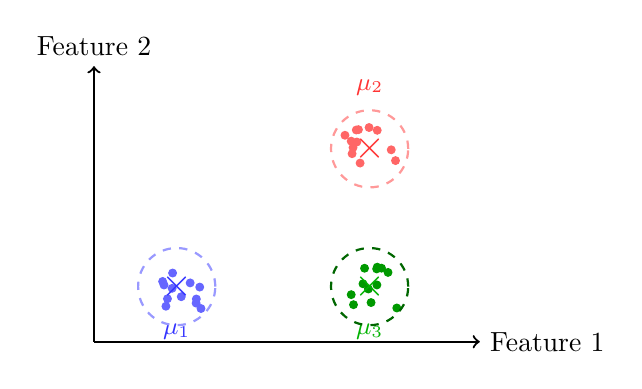
\begin{tikzpicture}[scale=0.7]
    % Cluster 1 (bottom-left) - Blue
    \foreach \i in {1,...,12} {
        \pgfmathsetmacro{\x}{1.5 + 0.5*rand}
        \pgfmathsetmacro{\y}{1 + 0.4*rand}
        \filldraw[blue!60] (\x, \y) circle (2pt);
    }
    \node[blue!80, font=\Large] at (1.5, 1) {$\times$};
    \node[blue!80, font=\small, below] at (1.5, 0.5) {$\mu_1$};
    \draw[blue!40, thick, dashed] (1.5, 1) circle (0.7cm);
    
    % Cluster 2 (top-right) - Red
    \foreach \i in {1,...,12} {
        \pgfmathsetmacro{\x}{5 + 0.5*rand}
        \pgfmathsetmacro{\y}{3.5 + 0.4*rand}
        \filldraw[red!60] (\x, \y) circle (2pt);
    }
    \node[red!80, font=\Large] at (5, 3.5) {$\times$};
    \node[red!80, font=\small, above] at (5, 4.3) {$\mu_2$};
    \draw[red!40, thick, dashed] (5, 3.5) circle (0.7cm);
    
    % Cluster 3 (bottom-right) - Green
    \foreach \i in {1,...,12} {
        \pgfmathsetmacro{\x}{5 + 0.5*rand}
        \pgfmathsetmacro{\y}{1 + 0.4*rand}
        \filldraw[green!60!black] (\x, \y) circle (2pt);
    }
    \node[green!70!black, font=\Large] at (5, 1) {$\times$};
    \node[green!70!black, font=\small, below] at (5, 0.5) {$\mu_3$};
    \draw[green!40!black, thick, dashed] (5, 1) circle (0.7cm);
    
    % Axes
    \draw[->, thick] (0, 0) -- (7, 0) node[right] {Feature 1};
    \draw[->, thick] (0, 0) -- (0, 5) node[above] {Feature 2};
\end{tikzpicture}

\vspace{0.8em}
\begin{itemize}
\item Each cluster has a \textbf{center} (centroid) $\mu_k$ (marked with $\times$)
\item Points belong to their \textbf{nearest} center
\item Goal: Find centers that minimize total distance to assigned points
\end{itemize}

\end{frame}

% --- SLIDE 3: K-Means Algorithm ---
\begin{frame}{K-Means Algorithm}

\begin{tcolorbox}[colback=blue!5, colframe=blue!50, title=\textbf{K-Means Algorithm}]

\textbf{Input:} Data $\{x_1, x_2, \ldots, x_n\}$ and number of clusters $K$

\vspace{0.5em}
\textbf{Initialize:} Randomly place $K$ cluster centers $\mu_1, \mu_2, \ldots, \mu_K$

\vspace{0.5em}
\textbf{Repeat until convergence:}

\vspace{0.3em}
\begin{enumerate}
\item \textbf{Assignment Step:} For each point $x_i$, assign to nearest center
\[
c_i = \arg\min_{k=1,\ldots,K} \|x_i - \mu_k\|^2
\]
\small (find which center is closest)

\vspace{0.5em}
\item \textbf{Update Step:} Move each center to mean of assigned points
\[
\mu_k = \frac{1}{|C_k|} \sum_{i \in C_k} x_i
\]
\small (average all points in cluster $k$)
\end{enumerate}

\vspace{0.5em}
\textbf{Stop when:} Assignments don't change OR max iterations reached
\end{tcolorbox}

\end{frame}

% --- SLIDE 4: K-Means Step-by-Step Visualization ---
\begin{frame}{K-Means: Step-by-Step Example}

\centering
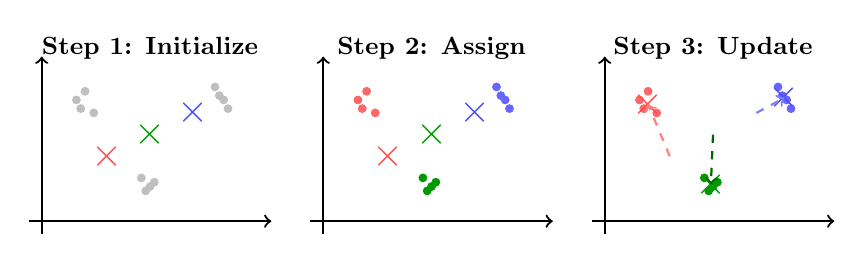
\begin{tikzpicture}[scale=0.55]
    % Step 1: Initial random centers
    \begin{scope}[shift={(0,0)}]
        \node[font=\small\bfseries] at (2.5, 4) {Step 1: Initialize};
        \draw[->, thick] (-0.3, 0) -- (5.3, 0);
        \draw[->, thick] (0, -0.3) -- (0, 3.8);
        
        % Data points (all gray initially)
        \foreach \x/\y in {0.8/2.8, 1.2/2.5, 1.0/3.0, 0.9/2.6,
                           4.2/2.8, 4.0/3.1, 4.3/2.6, 4.1/2.9,
                           2.5/0.8, 2.3/1.0, 2.6/0.9, 2.4/0.7} {
            \filldraw[gray!50] (\x, \y) circle (2.5pt);
        }
        
        % Random initial centers
        \node[red!70, font=\Large] at (1.5, 1.5) {$\times$};
        \node[blue!70, font=\Large] at (3.5, 2.5) {$\times$};
        \node[green!60!black, font=\Large] at (2.5, 2.0) {$\times$};
    \end{scope}
    
    % Step 2: Assign to nearest
    \begin{scope}[shift={(6.5,0)}]
        \node[font=\small\bfseries] at (2.5, 4) {Step 2: Assign};
        \draw[->, thick] (-0.3, 0) -- (5.3, 0);
        \draw[->, thick] (0, -0.3) -- (0, 3.8);
        
        % Points colored by assignment
        \foreach \x/\y in {0.8/2.8, 1.2/2.5, 1.0/3.0, 0.9/2.6} {
            \filldraw[red!60] (\x, \y) circle (2.5pt);
        }
        \foreach \x/\y in {4.2/2.8, 4.0/3.1, 4.3/2.6, 4.1/2.9} {
            \filldraw[blue!60] (\x, \y) circle (2.5pt);
        }
        \foreach \x/\y in {2.5/0.8, 2.3/1.0, 2.6/0.9, 2.4/0.7} {
            \filldraw[green!60!black] (\x, \y) circle (2.5pt);
        }
        
        % Old centers
        \node[red!70, font=\Large] at (1.5, 1.5) {$\times$};
        \node[blue!70, font=\Large] at (3.5, 2.5) {$\times$};
        \node[green!60!black, font=\Large] at (2.5, 2.0) {$\times$};
    \end{scope}
    
    % Step 3: Update centers
    \begin{scope}[shift={(13,0)}]
        \node[font=\small\bfseries] at (2.5, 4) {Step 3: Update};
        \draw[->, thick] (-0.3, 0) -- (5.3, 0);
        \draw[->, thick] (0, -0.3) -- (0, 3.8);
        
        % Points (same as step 2)
        \foreach \x/\y in {0.8/2.8, 1.2/2.5, 1.0/3.0, 0.9/2.6} {
            \filldraw[red!60] (\x, \y) circle (2.5pt);
        }
        \foreach \x/\y in {4.2/2.8, 4.0/3.1, 4.3/2.6, 4.1/2.9} {
            \filldraw[blue!60] (\x, \y) circle (2.5pt);
        }
        \foreach \x/\y in {2.5/0.8, 2.3/1.0, 2.6/0.9, 2.4/0.7} {
            \filldraw[green!60!black] (\x, \y) circle (2.5pt);
        }
        
        % NEW centers (moved to cluster means)
        \node[red!70, font=\Large] at (1.0, 2.7) {$\times$};
        \node[blue!70, font=\Large] at (4.15, 2.85) {$\times$};
        \node[green!60!black, font=\Large] at (2.45, 0.85) {$\times$};
        
        % Arrows showing movement
        \draw[->, red!50, thick, dashed] (1.5, 1.5) -- (1.0, 2.7);
        \draw[->, blue!50, thick, dashed] (3.5, 2.5) -- (4.15, 2.85);
        \draw[->, green!40!black, thick, dashed] (2.5, 2.0) -- (2.45, 0.85);
    \end{scope}
\end{tikzpicture}

\vspace{0.8em}
\textbf{Repeat steps 2-3} until centers stop moving (typically 10-100 iterations)

\end{frame}

% --- SLIDE 5: Choosing K (Elbow Method) ---
\begin{frame}{How to Choose K?}

\textbf{Problem:} How many clusters should we use?

\vspace{0.5em}
\begin{columns}[c]
\begin{column}{1.0\textwidth}
\textbf{Elbow Method}

Plot "within-cluster sum of squares" (WCSS) vs $K$

\[
\text{WCSS} = \sum_{k=1}^K \sum_{i \in C_k} \|x_i - \mu_k\|^2
\]

\vspace{0.3em}
\centering
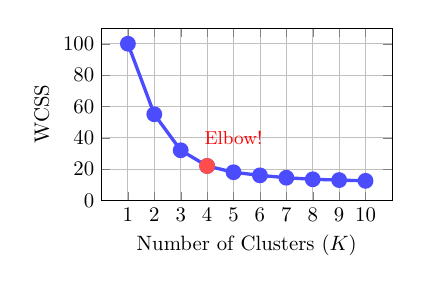
\begin{tikzpicture}[scale=0.75]
    \begin{axis}[
        width=6.5cm, height=4.5cm,
        xlabel={Number of Clusters ($K$)},
        ylabel={WCSS},
        grid=major,
        ymin=0, ymax=110,
        xmin=0, xmax=11,
        xtick={1,2,3,4,5,6,7,8,9,10},
        ytick={0,20,40,60,80,100}
    ]
    \addplot[blue!70, ultra thick, mark=*, mark size=3pt] coordinates {
        (1,100) (2,55) (3,32) (4,22) (5,18) (6,16) (7,14.5) (8,13.5) (9,13) (10,12.5)
    };
    \addplot[red!70, ultra thick, mark=*, mark size=3pt] coordinates {
        (4,22)
    };
    
    % Elbow annotation
    % \draw[red, very thick] (axis cs:2.5,20) -- (axis cs:4,20) -- (axis cs:4,35);
    \node[red, font=\small] at (axis cs:5,40) {Elbow!};
    % \draw[red, thick, ->] (axis cs:4.8,26) -- (axis cs:4,22);
    \end{axis}
\end{tikzpicture}

\vspace{0.3em}
\small Look for the "elbow" where adding more clusters doesn't help much (in the above case it is 4)
\end{column}

\end{columns}

\end{frame}

% --- SLIDE 7: Application 1 - Customer Segmentation ---
\begin{frame}{Application 1: Customer Segmentation}

\textbf{Use case:} Group customers for targeted marketing
\vspace{0.5em}

\begin{columns}[T] % align columns at the top

% ===================== LEFT COLUMN (Data & Plot) =====================
\begin{column}{0.48\textwidth}

    % Example Box
    \begin{tcolorbox}[
      colback=blue!5, colframe=blue!50,
      title=\textbf{Example: E-commerce Data},
      boxsep=3pt, left=4pt, right=4pt, top=3pt, bottom=3pt
    ]
    \small
    \begin{itemize}\setlength\itemsep{0.2em}
        \item Features: frequency, spend, recency
        \item Run K-Means with $K=4$
        \item Interpret clusters
    \end{itemize}
    \end{tcolorbox}

    \vspace{0.5em}
    
    % Scatter Plot
    \centering
    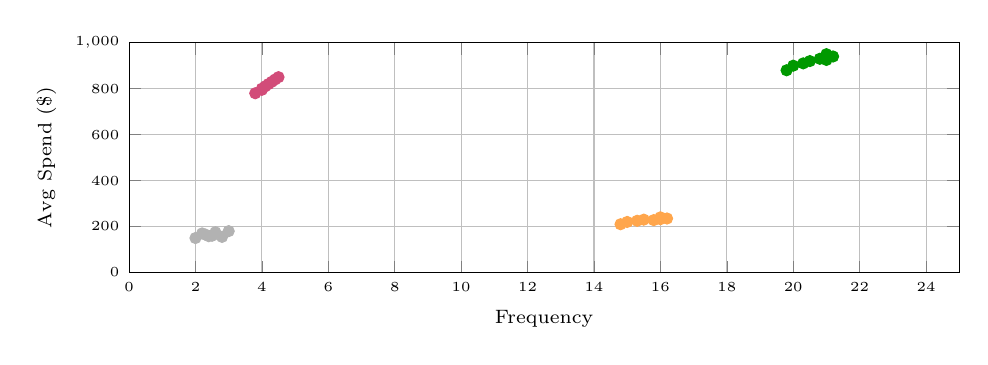
\begin{tikzpicture}
    \begin{axis}[
        width=\linewidth, height=4.5cm,
        xlabel={\scriptsize Frequency},
        ylabel={\scriptsize Avg Spend (\$)},
        grid=major,
        tick label style={font=\tiny},
        label style={font=\scriptsize},
        % legend style={font=\tiny, at={(0.02,0.98)}, anchor=north middle, fill opacity=0.8, draw=gray!20},
        xmin=0, xmax=25,
        ymin=0, ymax=1000
    ]
    % Inactive (Gray)
    \addplot[only marks, mark=*, mark size=2pt, gray!60] coordinates {
        (2,150) (3,180) (2.5,160) (2.2,170) (2.8,155)
        (2.3,165) (2.6,175) (2.4,158)
    };
    % Bargain (Orange)
    \addplot[only marks, mark=*, mark size=2pt, orange!70] coordinates {
        (15,220) (16,240) (15.5,230) (14.8,210) (16.2,235)
        (15.3,225) (15.8,228) (16,232)
    };
    % Big Spender (Purple)
    \addplot[only marks, mark=*, mark size=2pt, purple!70] coordinates {
        (4,800) (4.5,850) (4.2,820) (3.8,780) (4.3,830)
        (4.1,810) (4.4,840) (4.0,795)
    };
    % VIP (Green)
    \addplot[only marks, mark=*, mark size=2pt, green!60!black] coordinates {
        (20,900) (21,950) (20.5,920) (19.8,880) (21.2,940)
        (20.3,910) (20.8,930) (21,925)
    };
    % \legend{Inactive,Bargain,Big Spender,VIP}
    \end{axis}
    \end{tikzpicture}

\end{column}

% ===================== RIGHT COLUMN (Segments) =====================
\begin{column}{0.48\textwidth}
    \textbf{Discovered Segments:}
    \vspace{0.35em}

    % Inner Columns for the 2x2 grid
    \begin{columns}[T]
    
        % -- Inner Left --
        \begin{column}{0.48\textwidth}
            % Inactive Box
            \begin{tcolorbox}[colback=gray!10, colframe=gray!55,
              title=\centering\small\textbf{Inactive}, boxsep=2pt, left=2pt, right=2pt, top=2pt, bottom=2pt, height=2.4cm]
            \centering\small
            Low freq, \\low spend
            \vspace{0.3em}
            
            \textbf{Action:} \\Re-engage
            \end{tcolorbox}
            
            \vspace{0.3em}
            
            % Big Spender Box
            \begin{tcolorbox}[colback=purple!10, colframe=purple!55,
              title=\centering\small\textbf{Big Spenders}, boxsep=2pt, left=2pt, right=2pt, top=2pt, bottom=2pt, height=2.8cm]
            \centering\small
            Low freq, \\high spend
            \vspace{0.3em}
            
            \textbf{Action:} \\Premium Service
            \end{tcolorbox}
        \end{column}

        % -- Inner Right --
        \begin{column}{0.48\textwidth}
            % Bargain Box
            \begin{tcolorbox}[colback=orange!10, colframe=orange!55,
              title=\centering\small\textbf{Bargain}, boxsep=2pt, left=2pt, right=2pt, top=2pt, bottom=2pt, height=2.4cm]
            \centering\small
            High freq, \\low spend
            \vspace{0.3em}
            
            \textbf{Action:} \\Discounts
            \end{tcolorbox}
            
            \vspace{0.3em}
            
            % VIP Box
            \begin{tcolorbox}[colback=green!10, colframe=green!50!black,
              title=\centering\small\textbf{VIP}, boxsep=2pt, left=2pt, right=2pt, top=2pt, bottom=2pt, height=2.8cm]
            \centering\small
            High freq, \\high spend
            \vspace{0.3em}
            
            \textbf{Action:} \\Loyalty Program
            \end{tcolorbox}
        \end{column}
    \end{columns}
\end{column}

\end{columns}
\end{frame}
% --- SLIDE 8: Application 2 - Document Clustering (Simplified) ---
\begin{frame}{Application 2: Document Clustering}

\textbf{Use case:} Automatically organize news articles by topic.

% \vspace{1em}
\centering
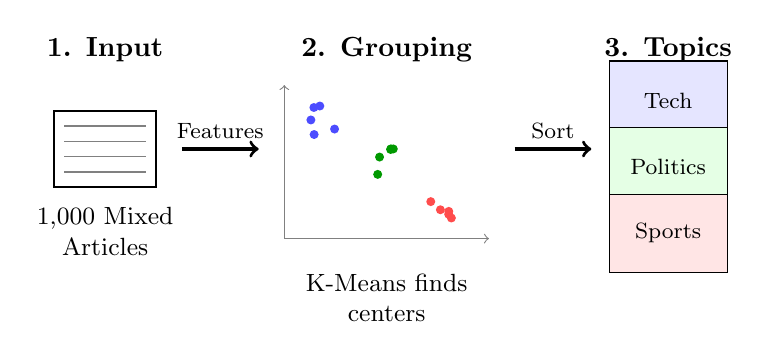
\begin{tikzpicture}[scale=0.65]
    % --- Step 1: Raw Documents (Left) ---
    \node[font=\bfseries] at (1, 4.2) {1. Input};
    
    % Simple document icons
    \draw[fill=white, thick] (0, 1.5) rectangle (2, 3);
    \foreach \y in {2.7, 2.4, 2.1, 1.8} {
        \draw[gray] (0.2, \y) -- (1.8, \y);
    }
    \node[below, align=center, font=\small] at (1, 1.3) {1,000 Mixed\\Articles};

    % Arrow 1
    \draw[->, very thick] (2.5, 2.25) -- (4, 2.25) node[midway, above, font=\footnotesize] {Features};

    % --- Step 2: Feature Space (Middle) ---
    \node[font=\bfseries] at (6.5, 4.2) {2. Grouping};
    
    % Axes
    \draw[->, gray] (4.5, 0.5) -- (8.5, 0.5);
    \draw[->, gray] (4.5, 0.5) -- (4.5, 3.5);

    % Clusters (simplified points)
    \foreach \i in {1,...,5} \fill[red!70] (7.5 + 0.3*rand, 1.2 + 0.3*rand) circle (2.5pt); % Sports
    \foreach \i in {1,...,5} \fill[blue!70] (5.2 + 0.3*rand, 2.8 + 0.3*rand) circle (2.5pt); % Tech
    \foreach \i in {1,...,5} \fill[green!60!black] (6.5 + 0.3*rand, 2.0 + 0.3*rand) circle (2.5pt); % Politics
    
    \node[below, align=center, font=\small] at (6.5, 0) {K-Means finds\\centers};

    % Arrow 2
    \draw[->, very thick] (9, 2.25) -- (10.5, 2.25) node[midway, above, font=\footnotesize] {Sort};

    % --- Step 3: Topics (Right) ---
    \node[font=\bfseries] at (12, 4.2) {3. Topics};

    % Folder Icons
    \node[draw, fill=blue!10, minimum width=1.5cm, minimum height=1cm, align=center, font=\footnotesize] at (12, 3.2) {Tech};
    \node[draw, fill=green!10, minimum width=1.5cm, minimum height=1cm, align=center, font=\footnotesize] at (12, 1.9) {Politics};
    \node[draw, fill=red!10, minimum width=1.5cm, minimum height=1cm, align=center, font=\footnotesize] at (12, 0.6) {Sports};

\end{tikzpicture}

% \vspace{1em}
\begin{tcolorbox}[colback=yellow!5, colframe=orange!40, title=\textbf{Process}]
\begin{itemize}
    \item Convert text into numbers (Text Features).
    \item Similar stories appear close together in space.
    \item K-Means automatically groups them into topics.
\end{itemize}
\end{tcolorbox}

\centering
\small \textit{Example: Google News grouping stories from different sources.}

\end{frame}

% --- SLIDE 9: Limitations of K-Means ---
\begin{frame}{When K-Means Fails}

\textbf{K-Means assumes spherical, equal-sized clusters}

\vspace{0.5em}
\begin{columns}[t]
\begin{column}{0.48\textwidth}
\textbf{Problem 1: Non-spherical}

\vspace{0.3em}
\centering
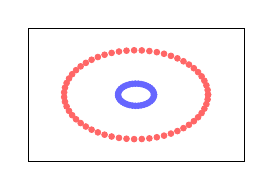
\begin{tikzpicture}[scale=0.7]
    \begin{axis}[
        width=5.5cm, height=4cm,
        grid=major,
        xmin=-3, xmax=3,
        ymin=-3, ymax=3,
        xtick=\empty, ytick=\empty
    ]
    
    % Two concentric circles
    \addplot[only marks, mark=*, mark size=1.5pt, blue!60, samples=40, domain=0:360] 
        ({0.5*cos(x)}, {0.5*sin(x)});
    \addplot[only marks, mark=*, mark size=1.5pt, red!60, samples=60, domain=0:360] 
        ({2*cos(x)}, {2*sin(x)});
    
    \end{axis}
\end{tikzpicture}

\vspace{0.2em}
\small {\color{red} Fails on concentric circles!}
\end{column}

\begin{column}{0.48\textwidth}
\textbf{Problem 2: Different sizes}

\vspace{0.3em}
\centering
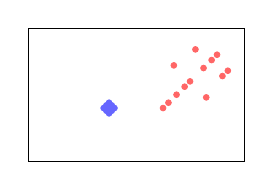
\begin{tikzpicture}[scale=0.7]
    \begin{axis}[
        width=5.5cm, height=4cm,
        grid=major,
        xmin=-3, xmax=5,
        ymin=-2, ymax=3,
        xtick=\empty, ytick=\empty
    ]
    
    % Small tight cluster
    \addplot[only marks, mark=*, mark size=1.5pt, blue!60] coordinates {
        (0,0) (0.1,0.1) (-0.1,0.1) (0.1,-0.1) (-0.1,-0.1)
        (0.2,0) (0,0.2) (-0.2,0) (0,-0.2)
    };
    
    % Large spread cluster
    \addplot[only marks, mark=*, mark size=1.5pt, red!60] coordinates {
        (3,1) (3.5,1.5) (2.5,0.5) (4,2) (2,0)
        (3.8,1.8) (2.2,0.2) (4.2,1.2) (2.8,0.8)
        (3.2,2.2) (3.6,0.4) (2.4,1.6) (4.4,1.4)
    };
    
    \end{axis}
\end{tikzpicture}

\vspace{0.2em}
\small {\color{red} Struggles with size differences!}
\end{column}
\end{columns}

\vspace{0.5em}
\begin{tcolorbox}[colback=yellow!8, colframe=orange!60, title=\textbf{Other Limitations}]
\begin{itemize}
\item Sensitive to outliers
\item Must specify $K$ in advance
\item Random initialization matters
\item Bad results for high dimensional data
\end{itemize}
\end{tcolorbox}

\vspace{0.3em}
\textbf{Alternatives:} DBSCAN (density-based), Gaussian Mixture Models, Hierarchical clustering

\end{frame}
% =========================
% PCA (Principal Component Analysis) - IMPROVED VERSION
% =========================

\section{Dimensionality Reduction: PCA}

% --- SLIDE 1: The Curse of Dimensionality ---
\begin{frame}{The Curse of Dimensionality}

\textbf{Real-world data is high-dimensional:}

\vspace{0.8em}
\begin{columns}[c]
\begin{column}{0.48\textwidth}
\textbf{Examples:}
\begin{itemize}
\item Images: 1000$\times$1000 = 1M pixels
\item Text: 10,000+ words
\item Genomics: 20,000+ genes
\item Sensors: 100+ measurements
\end{itemize}

\vspace{1em}
\textbf{Problems:}
\begin{itemize}
\item Hard to visualize
\item Slow to compute
\item Lots of redundancy
\item Noisy measurements
\end{itemize}
\end{column}

\begin{column}{0.48\textwidth}
\centering
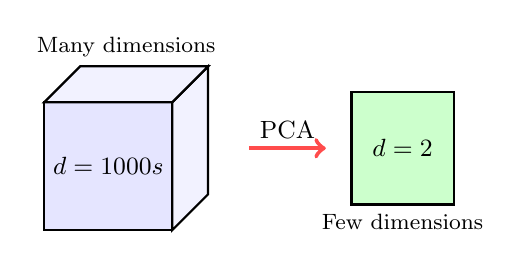
\begin{tikzpicture}[scale=0.65]
    % 3D cube representing high dimensions
    \draw[thick, fill=blue!10] (0,0) rectangle (2.5,2.5);
    \draw[thick, fill=blue!5] (2.5,0) -- (3.2,0.7) -- (3.2,3.2) -- (2.5,2.5) -- cycle;
    \draw[thick, fill=blue!5] (0,2.5) -- (0.7,3.2) -- (3.2,3.2) -- (2.5,2.5) -- cycle;
    
    \node at (1.25, 1.25) {\small $d = 1000s$};
    \node[above, font=\footnotesize] at (1.6, 3.2) {Many dimensions};
    
    % Arrow
    \draw[->, ultra thick, red!70] (4, 1.6) -- (5.5, 1.6);
    \node[above, font=\small] at (4.75, 1.6) {PCA};
    
    % 2D plane representing low dimensions
    \draw[thick, fill=green!20] (6,0.5) rectangle (8,2.7);
    \node at (7, 1.6) {\small $d = 2$};
    \node[below, font=\footnotesize] at (7, 0.5) {Few dimensions};
\end{tikzpicture}

\vspace{1em}
\textbf{Solution:}
Find a lower-dimensional representation while keeping important information (Dimensionality Reduction)
\end{column}
\end{columns}

\end{frame}

% --- SLIDE 2: What is PCA? ---
\begin{frame}{What is PCA?}

\textbf{Principal Component Analysis (PCA)} is a dimensionality reduction algorithm that finds the most important directions in your data.

\vspace{1em}
\begin{tcolorbox}[colback=blue!5, colframe=blue!50, title=\textbf{Core Idea}]
Instead of using original features, create \textbf{new features} (principal components) that:
\begin{itemize}
\item Capture maximum variance
\item Are uncorrelated with each other
\item Are ranked by importance
\end{itemize}

Then keep only the top few components!
\end{tcolorbox}

\vspace{1em}
\centering
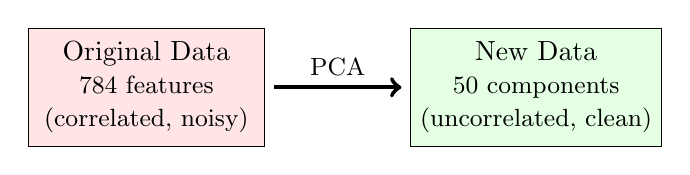
\begin{tikzpicture}[scale=0.9]
    \node[draw, rectangle, fill=red!10, minimum width=3cm, minimum height=1.5cm, align=center] at (0,0) {
        Original Data\\
        \small 784 features\\
        \small (correlated, noisy)
    };
    
    \draw[->, ultra thick] (1.8, 0) -- (3.6, 0) node[midway, above] {\small PCA};
    
    \node[draw, rectangle, fill=green!10, minimum width=3cm, minimum height=1.5cm, align=center] at (5.5,0) {
        New Data\\
        \small 50 components\\
        \small (uncorrelated, clean)
    };
\end{tikzpicture}

\end{frame}

% --- SLIDE 3: PCA Intuition - Finding Directions ---
\begin{frame}{PCA Intuition: Finding the Best Directions}

\textbf{Goal:} Find directions where data varies the most.

\vspace{0.5em}
\centering
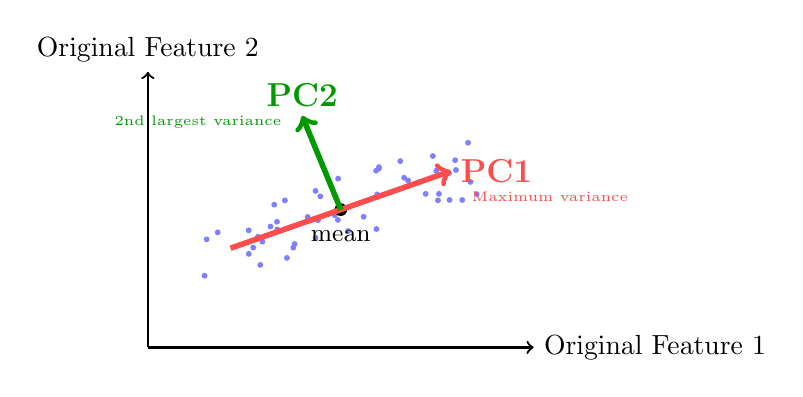
\begin{tikzpicture}[scale=0.7]
    % Data points (elongated cloud)
    \foreach \i in {1,...,50} {
        \pgfmathsetmacro{\x}{2.5*rand + 3.5}
        \pgfmathsetmacro{\y}{0.6*rand + 2.5 + 0.35*(\x-3.5)}
        \filldraw[blue!50] (\x, \y) circle (1.2pt);
    }
    
    % Mean point
    \filldraw[black] (3.5, 2.5) circle (3pt);
    \node[below] at (3.5, 2.3) {\small mean};
    
    % First principal component (main direction of variance)
    \draw[->, red!70, ultra thick, line width=2pt] (1.5, 1.8) -- (5.5, 3.2);
    \node[red!70, font=\large, right] at (5.5, 3.2) {\textbf{PC1}};
    \node[red!70, font=\tiny, below right] at (5.7, 3.0) {Maximum variance};
    
    % Second principal component (orthogonal)
    \draw[->, green!60!black, ultra thick, line width=2pt] (3.5, 2.5) -- (2.8, 4.2);
    \node[green!60!black, font=\large, above] at (2.8, 4.2) {\textbf{PC2}};
    \node[green!60!black, font=\tiny, above left] at (2.6, 3.8) {2nd largest variance};
    
    % Axes
    \draw[->, thick] (0, 0) -- (7, 0) node[right] {Original Feature 1};
    \draw[->, thick] (0, 0) -- (0, 5) node[above] {Original Feature 2};
\end{tikzpicture}

\vspace{0.8em}
\begin{itemize}
\item PC1: Direction with most spread
\item PC2: Perpendicular to PC1, next most spread
\item PC3, PC4, ... : Each perpendicular to all previous ones
\end{itemize}

\end{frame}

% --- SLIDE 4a: How Does PCA Work? (Part 1) ---
\begin{frame}{How Does PCA Work? (Part 1)}

\textbf{Step 1: Prepare the Data}

% \vspace{0.8em}
\begin{tcolorbox}[colback=gray!5, colframe=gray!80, title=\textbf{1. Center the Data}]
Shift the data so the center is at the origin (0,0).
% \vspace{0.5em}
\[
X_{\text{centered}} = X - \bar{X}
\]
\small \textit{(Subtract the mean from every feature)}
\end{tcolorbox}

% \vspace{1em}
\begin{tcolorbox}[colback=blue!5, colframe=blue!50, title=\textbf{2. Compute Covariance Matrix}]
Calculate how features vary with respect to each other.
\vspace{0.5em}
\[
C = \frac{1}{n} X_{\text{centered}}^\top X_{\text{centered}}
\]
\small \textit{(Finds correlations between features)}
\end{tcolorbox}

\end{frame}

% --- SLIDE 4b: How Does PCA Work? (Part 2) ---
\begin{frame}{How Does PCA Work? (Part 2)}

\textbf{Step 2: Find Directions \& Project}

% \vspace{0.8em}
\begin{tcolorbox}[colback=purple!5, colframe=purple!50, title=\textbf{3. Find Principal Components}]
Calculate \textbf{Eigenvectors} and \textbf{Eigenvalues} of the covariance matrix $C$.
\begin{itemize}
    \item \textbf{Eigenvectors:} The directions of the new axes.
    \item \textbf{Eigenvalues:} The amount of variance (information) along those axes.
\end{itemize}
\end{tcolorbox}

% \vspace{1em}
\begin{tcolorbox}[colback=red!5, colframe=red!50, title=\textbf{4. Select \& Project}]
Pick the top $k$ eigenvectors with the largest eigenvalues and transform the data.
\vspace{0.5em}
\[
Z = X_{\text{centered}} \cdot V_k
\]
\small \textit{(Reduces data from $d$ dimensions $\rightarrow$ $k$ dimensions)}
\end{tcolorbox}

\end{frame}

% --- SLIDE 6: Choosing Number of Components ---
\begin{frame}{How Many Components to Keep?}

\textbf{Key question:} How many components are enough?

\vspace{0.5em}
\centering
\textbf{Cumulative Variance Explained}

% \vspace{0.2em}
{\small (The most common method for selecting $K$)}

% \vspace{1em}
\centering
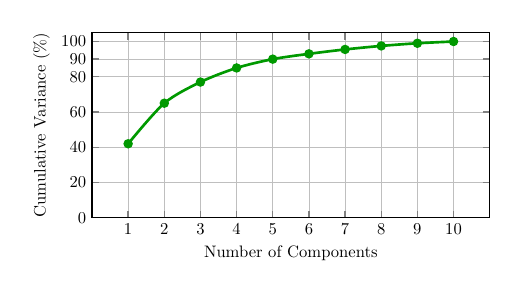
\begin{tikzpicture}[scale=0.6]
    \begin{axis}[
        width=10cm, height=5.5cm, % Made wider since it's alone now
        xlabel={Number of Components},
        ylabel={Cumulative Variance (\%)},
        grid=major,
        ymin=0, ymax=105,
        xmin=0, xmax=11,
        xtick={1,2,3,4,5,6,7,8,9,10},
        ytick={0,20,40,60,80,90,100},
        axis line style={thick},
        tick style={thick}
    ]
    % Cumulative Curve
    \addplot[green!60!black, ultra thick, mark=*, smooth] coordinates {
        (1,42) (2,65) (3,77) (4,85) (5,90) (6,93) (7,95.5) (8,97.5) (9,99) (10,100)
    };
    
    % % 90% Threshold Line
    % \draw[red, thick, dashed] (axis cs:0,90) -- (axis cs:11,90);
    % \node[red, font=\small, above] at (axis cs:2.5,90) {Target Threshold (e.g., 90\%)};
    
    % % Dropdown line showing K=5 hits the target
    % \draw[red, thick, dashed] (axis cs:5,0) -- (axis cs:5,90);
    % \node[red, font=\bfseries] at (axis cs:5.2, 85) {Select $K=5$};
    % \filldraw[red] (axis cs:5,90) circle (2.5pt);

    \end{axis}
\end{tikzpicture}

% \vspace{1em}
\begin{tcolorbox}[colback=blue!5, colframe=blue!50, width=0.9\linewidth]
\textbf{Rule of Thumb:} Choose the smallest $K$ that preserves \textbf{80--95\%} of the total variance.
\end{tcolorbox}

\end{frame}


% --- SLIDE 7a: MNIST Case Study (The Data) ---
\begin{frame}{Application 1: Data Visualization}

\textbf{The Data:} MNIST Digits, 70,000 handwritten digits (0--9).

\vspace{1em}
\begin{columns}[c]
\begin{column}{0.45\textwidth}
\textbf{The Challenge:}
\begin{itemize}
    \item Each image is $28 \times 28$ pixels.
    \item Total features: $28 \times 28 = \mathbf{784}$ dimensions!
    \item We cannot "see" in 784 dimensions.
\end{itemize}

\vspace{1em}
\textbf{Question:} Can we compress this to just \textbf{2D} to see how the digits relate?
\end{column}

\begin{column}{0.5\textwidth}
\centering
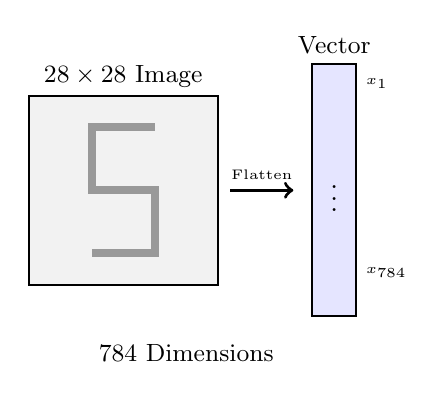
\begin{tikzpicture}[scale=0.8]
    % 2D Image Grid
    \draw[thick, fill=gray!10] (0,0) rectangle (3,3);
    \node at (1.5, 3.3) {\small $28 \times 28$ Image};
    
    % Draw a "Digit 5" roughly
    \draw[line width=3pt, gray!80] (2, 2.5) -- (1, 2.5) -- (1, 1.5) -- (2, 1.5) -- (2, 0.5) -- (1, 0.5);

    % Arrow
    \draw[->, very thick] (3.2, 1.5) -- (4.2, 1.5) node[midway, above, font=\tiny] {Flatten};

    % High-D Vector
    \draw[thick, fill=blue!10] (4.5, -0.5) rectangle (5.2, 3.5);
    \node at (4.85, 3.8) {\small Vector};
    \node at (4.85, 1.5) {\vdots};
    \node[right, font=\tiny] at (5.2, 3.2) {$x_1$};
    \node[right, font=\tiny] at (5.2, 0.2) {$x_{784}$};
    
    \node[below, align=center, font=\small] at (2.5, -0.8) {784 Dimensions};
\end{tikzpicture}
\end{column}
\end{columns}

\end{frame}

% --- SLIDE 7b: MNIST PCA Result ---
\begin{frame}{Application 1: Data Visualization}

\textbf{Applying PCA:} We project the 784 dimensions down to the top 2 Principal Components.

\vspace{0.5em}
\centering

\begin{figure}
    \centering
    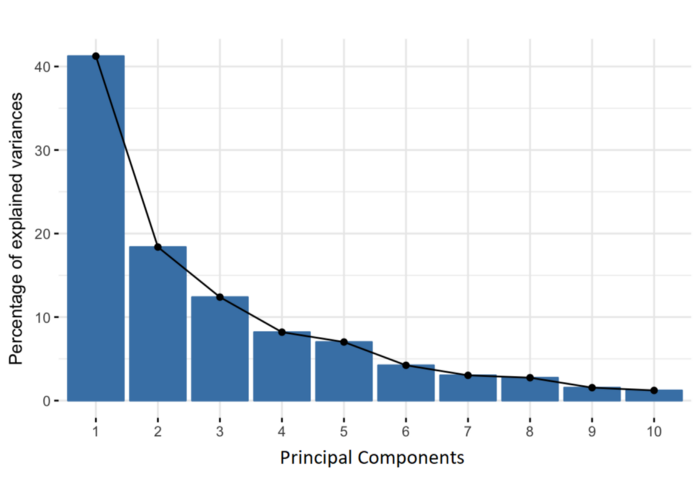
\includegraphics[width=0.8\linewidth]{images/PCA_Explained_VAR_MNIST.png}
    \label{fig:placeholder}
\end{figure}
\end{frame}

% --- SLIDE 7b: MNIST PCA Result ---
% --- SLIDE 7b: MNIST PCA Result & Critique ---
\begin{frame}{Application 1: Data Visualization}

\begin{columns}[c]
% --- LEFT COLUMN: Analysis ---
\begin{column}{0.45\textwidth}
    \textbf{Is this the best visualization?}
    
    \vspace{0.5em}
    \begin{itemize}
        \item It captures some structure, but points overlap heavily.
        \item \textbf{Reason:} PCA is \textbf{linear}, it cannot unfold complex, curved structures. 
        \item PCA is mostly used for compression. We will cover a better visualization algorithm shortly.
    \end{itemize}

\end{column}

% --- RIGHT COLUMN: Image ---
\begin{column}{0.55\textwidth}
    \centering
    % Ensure you have the file 'PCA_MNIST.png' in your project folder
    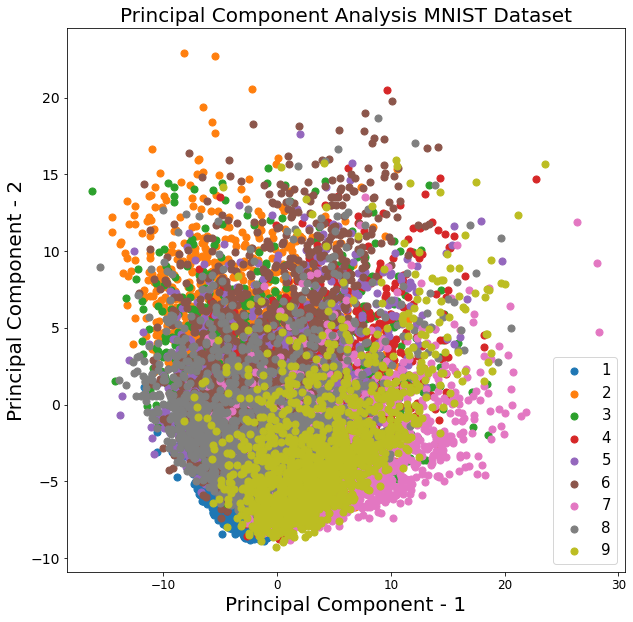
\includegraphics[width=\linewidth]{images/PCA_MNIST.png}
\end{column}
\end{columns}

\end{frame}
% --- SLIDE 8: Application 2 - Compression & Reconstruction ---
\begin{frame}{Application 2: Data Compression}

\textbf{Use case:} Store data more efficiently

\vspace{0.25em}
\centering
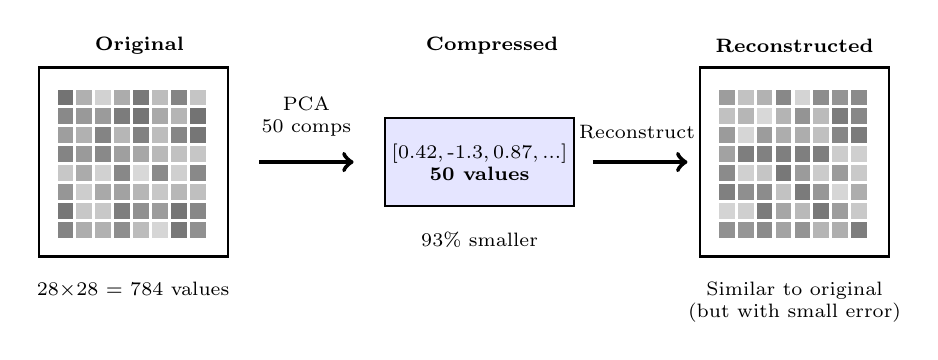
\begin{tikzpicture}[scale=0.80] % was 0.83
    % Original image
    \node[font=\scriptsize\bfseries] at (1.6, 3.35) {Original}; % slightly lower + smaller
    \draw[thick] (0,0) rectangle (3,3);
    \foreach \i in {0.3,0.6,...,2.7} {
        \foreach \j in {0.3,0.6,...,2.7} {
            \pgfmathsetmacro{\shade}{15 + 40*rnd}
            \fill[black!\shade] (\i,\j) rectangle +(0.25,0.25);
        }
    }
    \node[below, font=\scriptsize] at (1.5, -0.25) {28$\times$28 = 784 values}; % smaller

    % Arrow and compression info
    \draw[->, ultra thick] (3.5, 1.5) -- (5, 1.5);
    \node[above, font=\scriptsize, align=center] at (4.25, 1.75) {PCA\\50 comps}; % shorter text

    % Compressed representation
    \node[font=\scriptsize\bfseries] at (7.2, 3.35) {Compressed};
    \draw[thick, fill=blue!10] (5.5,0.8) rectangle (8.5,2.2);
    \node[align=center, font=\scriptsize] at (7, 1.5) {%
        [0.42,\,-1.3,\,0.87,\,...]\\
        \textbf{50 values}
    };
    \node[below, font=\scriptsize] at (7, 0.55) {93\% smaller};

    % Arrow back
    \draw[->, ultra thick] (8.8, 1.5) -- (10.3, 1.5);
    \node[above, font=\scriptsize] at (9.50, 1.72) {Reconstruct};

    % Reconstructed image
    \node[font=\scriptsize\bfseries] at (12, 3.35) {Reconstructed};
    \draw[thick] (10.5,0) rectangle (13.5,3);
    \foreach \i in {0.3,0.6,...,2.7} {
        \foreach \j in {0.3,0.6,...,2.7} {
            \pgfmathsetmacro{\shade}{15 + 38*rnd}
            \fill[black!\shade] (10.5+\i,\j) rectangle +(0.25,0.25);
        }
    }
    \node[below, font=\scriptsize, align=center] at (12, -0.25) {Similar to original\\(but with small error)};
\end{tikzpicture}

\vspace{0.15em}
\centering
\small \textbf{More components = better reconstruction, less compression}

\vspace{0.35em}
\begin{columns}[c]
\begin{column}{0.32\textwidth}
\centering
\small \textbf{10 PCs}\\99\% compression \\(blurry)
\end{column}
\begin{column}{0.32\textwidth}
\centering
\small \textbf{50 PCs}\\93\% compression \\(good)
\end{column}
\begin{column}{0.32\textwidth}
\centering
\small \textbf{200 PCs}\\75\% compression \\(near perfect)
\end{column}
\end{columns}

\end{frame}


% --- SLIDE 10: PCA Limitations ---
\begin{frame}{PCA Limitations}

\begin{columns}[c]
\begin{column}{1.0\textwidth}
\textbf{PCA Limitations:}

\begin{itemize}
\item \textbf{Linear only}: Finds linear combinations of features
\item \textbf{Sensitive to scale}: Must standardize data first
\item \textbf{Not Interpretable}: PCs are combinations of all features
\item \textbf{Outliers}: Can distort principal components
\end{itemize}

\end{column}
\end{columns}

\vspace{1em}
\centering
\small \textit{Let's have a look at a better algorithm for high dimensional data visualization...}

\end{frame}



% =========================
% t-SNE (Intuition Only)
% =========================

\section{Dimensionality Reduction: t-SNE}

% --- SLIDE: Why t-SNE? ---
\begin{frame}{t-SNE: Why Do We Need It?}

\textbf{PCA is great... but it's linear.} Many datasets have \textbf{non-linear} structure.

\vspace{0.8em}
\begin{columns}[c]
\begin{column}{1.0\textwidth}
\begin{tcolorbox}[colback=blue!5, colframe=blue!50, title=\textbf{Problem}]
\begin{itemize}
\item High-dimensional data can be hard to visualize
\item PCA may \textbf{mix} classes if the separation is non-linear
\item We mainly want a \textbf{good 2D plot} for exploration
\end{itemize}
\end{tcolorbox}
\end{column}
\end{columns}

\end{frame}


% --- SLIDE: t-SNE intuition (no math) ---
\begin{frame}{t-Distributed Stochastic Neighbor Embedding (t-SNE)}

\begin{tcolorbox}[colback=yellow!8, colframe=orange!60, title=\textbf{Main Idea}]
t-SNE tries to build a 2D map where:
neighbors in high-D remain neighbors in 2D.
\end{tcolorbox}

\vspace{0.8em}
\begin{columns}[c]

\begin{column}{1.0\textwidth}
\centering
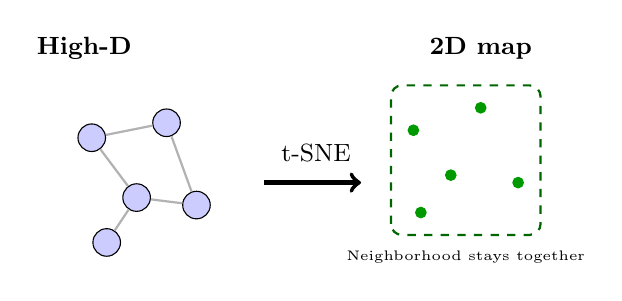
\begin{tikzpicture}[scale=0.95]
    % Left: high-D as a "neighborhood graph"
    \node[font=\small\bfseries] at (-0.1,3.2) {High-D};
    \foreach \p/\x/\y in {a/0/2, b/1/2.2, c/0.6/1.2, d/1.4/1.1, e/0.2/0.6} {
        \node[circle, draw, fill=blue!20, minimum size=0.35cm] (\p) at (\x,\y) {};
    }
    \draw[thick, gray!60] (a)--(b);
    \draw[thick, gray!60] (a)--(c);
    \draw[thick, gray!60] (c)--(d);
    \draw[thick, gray!60] (c)--(e);
    \draw[thick, gray!60] (b)--(d);

    % Arrow
    \draw[->, ultra thick] (2.3,1.4) -- (3.6,1.4);
    \node[font=\small] at (3.0,1.8) {t-SNE};

    % Right: 2D
    \node[font=\small\bfseries] at (5.2,3.2) {2D map};
    \foreach \x/\y in {4.3/2.1, 5.2/2.4, 4.8/1.5, 5.7/1.4, 4.4/1.0} {
        \filldraw[green!60!black] (\x,\y) circle (2pt);
    }
    \draw[rounded corners, dashed, thick, green!40!black] (4.0,0.7) rectangle (6.0,2.7);
    \node[font=\tiny, align=center] at (5.0,0.4) {Neighborhood stays together};
\end{tikzpicture}
\end{column}
\end{columns}

\end{frame}


% --- SLIDE: Example (synthetic PCA-like vs t-SNE-like) ---
\begin{frame}{Example: Visualizing MNIST via t-SNE}
\begin{figure}
    \centering
    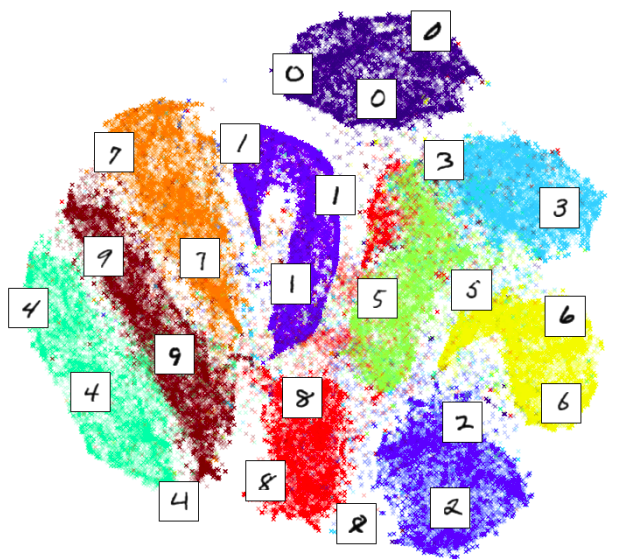
\includegraphics[width=0.65\linewidth]{images/tsne.png}
\end{figure}
\vspace{0.4em}
\centering
\small \textit{This is much better than PCA! We can see how similar digits are grouped together, while different ones are far from each other.}

\end{frame}








% --- SLIDE: Transition to Autoencoders ---
\begin{frame}[c]
\centering

We have covered classical algorithms like K-Means and PCA.

Now, let's explore a powerful Neural Network architecture designed for unsupervised learning...


\end{frame}


\section{Autoencoders}

% --- SLIDE 2: What is an Autoencoder? ---
\begin{frame}{What is an Autoencoder?}

\textbf{Autoencoder:} a type of neural network that learn to compress data into a compact form and then reconstruct it to match the original input.

% \hspace{0.2em}

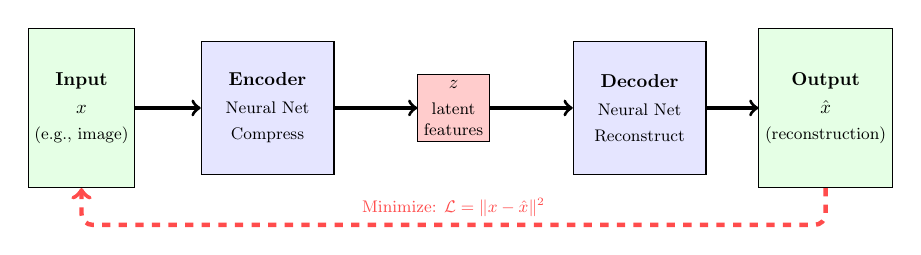
\begin{tikzpicture}[scale=0.675, transform shape]
     % Input
     \node[draw, rectangle, fill=green!10, minimum width=2cm, minimum height=3cm, align=center] (input) at (0,0) {
         \textbf{Input}\\[0.3em]
         $x$\\[0.2em]
         \small (e.g., image)
     };

     % Encoder
     \node[draw, rectangle, fill=blue!10, minimum width=2.5cm, minimum height=2.5cm, align=center] (encoder) at (3.5,0) {
         \textbf{Encoder}\\[0.3em]
         \small Neural Net\\[0.2em]
         \small Compress
     };

     % Latent/Bottleneck
     \node[draw, rectangle, fill=red!20, minimum width=1.2cm, minimum height=1.2cm, align=center] (latent) at (7,0) {
         \textbf{$z$}\\[0.2em]
         \small latent\\[-0.1em]
         \small features
     };

     % Decoder
     \node[draw, rectangle, fill=blue!10, minimum width=2.5cm, minimum height=2.5cm, align=center] (decoder) at (10.5,0) {
         \textbf{Decoder}\\[0.3em]
         \small Neural Net\\[0.2em]
         \small Reconstruct
     };

     % Output
     \node[draw, rectangle, fill=green!10, minimum width=2cm, minimum height=3cm, align=center] (output) at (14,0) {
         \textbf{Output}\\[0.3em]
         $\hat{x}$\\[0.2em]
         \small (reconstruction)
     };

     % Forward arrows
     \draw[->, very thick] (input) -- (encoder);
     \draw[->, very thick] (encoder) -- (latent);
     \draw[->, very thick] (latent) -- (decoder);
     \draw[->, very thick] (decoder) -- (output);

     % Loss arrow (Corrected: Squared path underneath)
     % Goes Down -> Left -> Up
     \draw[->, dashed, red!70, ultra thick, rounded corners] 
        (output.south) -- (14,-2.2) -- node[midway, above, font=\small] {Minimize: $\mathcal{L} = \|x - \hat{x}\|^2$} (0,-2.2) -- (input.south);

\end{tikzpicture}

\vspace{0.5em}
\textbf{The trick:} Force information through a narrow \textbf{bottleneck} $z$.

\vspace{0.2em}
\centering
\small This forces the network to learn compressed, meaningful representations!

\end{frame}

% --- SLIDE 3: Why Does This Work? ---
\begin{frame}{Why Does the Bottleneck Work?}
What if there's no bottleneck?

\vspace{1.5em}
\begin{columns}[c]
\begin{column}{0.48\textwidth}
\textbf{Without Bottleneck}

\vspace{0.3em}
\centering
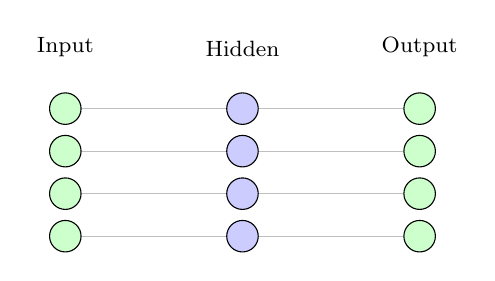
\begin{tikzpicture}[scale=0.9]
    % Input layer
    \foreach \i in {1,...,4} {
        \node[circle, draw, fill=green!20, minimum size=0.4cm] (i\i) at (0, -\i*0.6) {};
    }
    \node[above, font=\footnotesize] at (0, 0) {Input};
    
    % Hidden layer (same size)
    \foreach \i in {1,...,4} {
        \node[circle, draw, fill=blue!20, minimum size=0.4cm] (h\i) at (2.5, -\i*0.6) {};
    }
    \node[above, font=\footnotesize] at (2.5, 0) {Hidden};
    
    % Output layer
    \foreach \i in {1,...,4} {
        \node[circle, draw, fill=green!20, minimum size=0.4cm] (o\i) at (5, -\i*0.6) {};
    }
    \node[above, font=\footnotesize] at (5, 0) {Output};
    
    % Identity connections
    \foreach \i in {1,...,4} {
        \draw[gray!50] (i\i) -- (h\i) -- (o\i);
    }
\end{tikzpicture}

\vspace{0.3em}
\small Network can just copy:\\
$h_i = x_i$, $\hat{x}_i = h_i$

\vspace{0.3em}
{\color{red} Learns nothing useful!}
\end{column}

\begin{column}{0.48\textwidth}
\textbf{With Bottleneck}

\vspace{0.3em}
\centering
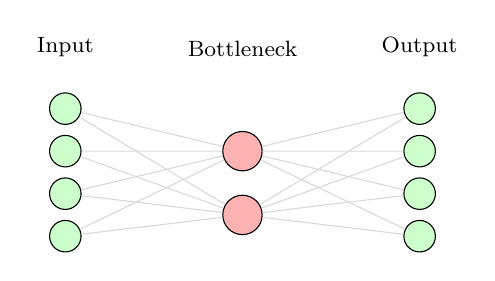
\begin{tikzpicture}[scale=0.9]
    % Input layer
    \foreach \i in {1,...,4} {
        \node[circle, draw, fill=green!20, minimum size=0.4cm] (i\i) at (0, -\i*0.6) {};
    }
    \node[above, font=\footnotesize] at (0, 0) {Input};
    
    % Bottleneck (smaller)
    \foreach \i in {1,2} {
        \node[circle, draw, fill=red!30, minimum size=0.5cm] (b\i) at (2.5, -\i*0.9-0.3) {};
    }
    \node[above, font=\footnotesize] at (2.5, 0) {Bottleneck};
    
    % Output layer
    \foreach \i in {1,...,4} {
        \node[circle, draw, fill=green!20, minimum size=0.4cm] (o\i) at (5, -\i*0.6) {};
    }
    \node[above, font=\footnotesize] at (5, 0) {Output};
    
    % Full connections
    \foreach \i in {1,...,4} {
        \foreach \j in {1,2} {
            \draw[gray!30] (i\i) -- (b\j);
            \draw[gray!30] (b\j) -- (o\i);
        }
    }
\end{tikzpicture}

\vspace{0.3em}
\small Must compress 4D $\rightarrow$ 2D\\
Forces learning of structure!

\vspace{0.3em}
{\color{green!60!black} Learns meaningful features!}
\end{column}
\end{columns}

\end{frame}

% --- SLIDE 7: Application 1 - Dimensionality Reduction ---% --- SLIDE 7: Application 1 - Dimensionality Reduction ---
\begin{frame}{Application 1: Dimensionality Reduction}

\textbf{How to use an Autoencoder for compression:}

\vspace{0.5em}
\centering
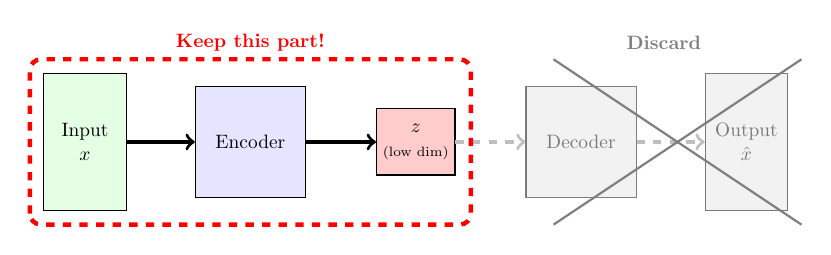
\begin{tikzpicture}[scale=0.7, transform shape]
    % Nodes
    \node[draw, rectangle, fill=green!10, minimum width=1.5cm, minimum height=2.5cm, align=center] (input) at (0,0) {Input\\$x$};
    
    \node[draw, rectangle, fill=blue!10, minimum width=2cm, minimum height=2cm, align=center] (encoder) at (3,0) {Encoder};
    
    \node[draw, rectangle, fill=red!20, minimum width=1.2cm, minimum height=1.2cm, align=center] (latent) at (6,0) {$z$\\\scriptsize(low dim)};
    
    \node[draw, rectangle, fill=gray!20, minimum width=2cm, minimum height=2cm, align=center, opacity=0.5] (decoder) at (9,0) {Decoder};
    
    \node[draw, rectangle, fill=gray!20, minimum width=1.5cm, minimum height=2.5cm, align=center, opacity=0.5] (output) at (12,0) {Output\\$\hat{x}$};
    
    % Arrows
    \draw[->, very thick] (input) -- (encoder);
    \draw[->, very thick] (encoder) -- (latent);
    \draw[->, very thick, gray!50, dashed] (latent) -- (decoder);
    \draw[->, very thick, gray!50, dashed] (decoder) -- (output);
    
    % Highlight Box (The Encoder Part)
    \draw[red, ultra thick, dashed, rounded corners] (-1, -1.5) rectangle (7, 1.5);
    \node[red, font=\bfseries] at (3, 1.8) {Keep this part!};
    
    % Discard label
    \node[gray, font=\bfseries] at (10.5, 1.8) {Discard};
    \draw[thick, gray] (8.5, -1.5) -- (13, 1.5);
    \draw[thick, gray] (8.5, 1.5) -- (13, -1.5);
\end{tikzpicture}

\vspace{1em}
\begin{tcolorbox}[colback=blue!5, colframe=blue!50, title=\textbf{The Process}]
\begin{enumerate}
    \item \textbf{Train} the full network to reconstruct the input ($x \approx \hat{x}$).
    \item \textbf{Discard} the Decoder (it's only needed for training).
    \item \textbf{Use the Encoder} to map high-dimensional data $x$ to low-dimensional code $z$.
\end{enumerate}
\end{tcolorbox}

\end{frame}

% --- SLIDE: Application - Image Generation ---
\begin{frame}{Application 2: Image Generation}

\textbf{How to use an Autoencoder for generation:}

\vspace{0.5em}
\centering
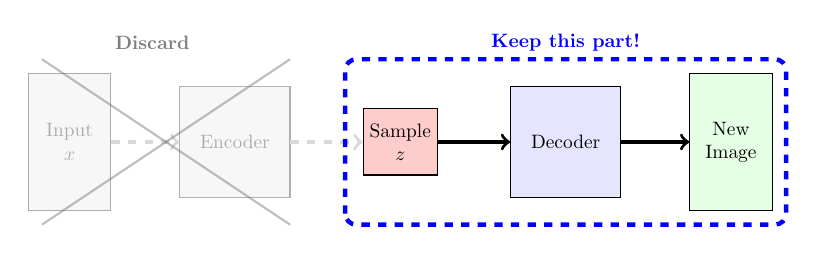
\begin{tikzpicture}[scale=0.7, transform shape]
    % Nodes (Ghosted Encoder side)
    \node[draw, rectangle, fill=gray!20, minimum width=1.5cm, minimum height=2.5cm, align=center, opacity=0.3] (input) at (0,0) {Input\\$x$};
    
    \node[draw, rectangle, fill=gray!20, minimum width=2cm, minimum height=2cm, align=center, opacity=0.3] (encoder) at (3,0) {Encoder};
    
    % Active Latent Code
    \node[draw, rectangle, fill=red!20, minimum width=1.2cm, minimum height=1.2cm, align=center] (latent) at (6,0) {Sample\\$z$};
    
    % Active Decoder side
    \node[draw, rectangle, fill=blue!10, minimum width=2cm, minimum height=2cm, align=center] (decoder) at (9,0) {Decoder};
    
    \node[draw, rectangle, fill=green!10, minimum width=1.5cm, minimum height=2.5cm, align=center] (output) at (12,0) {New\\Image};
    
    % Arrows
    \draw[->, very thick, gray!30, dashed] (input) -- (encoder);
    \draw[->, very thick, gray!30, dashed] (encoder) -- (latent);
    \draw[->, very thick] (latent) -- (decoder);
    \draw[->, very thick] (decoder) -- (output);
    
    % Highlight Box (The Decoder Part)
    \draw[blue, ultra thick, dashed, rounded corners] (5, -1.5) rectangle (13, 1.5);
    \node[blue, font=\bfseries] at (9, 1.8) {Keep this part!};
    
    % Discard label
    \node[gray, font=\bfseries] at (1.5, 1.8) {Discard};
    \draw[thick, gray, opacity=0.5] (-0.5, -1.5) -- (4, 1.5);
    \draw[thick, gray, opacity=0.5] (-0.5, 1.5) -- (4, -1.5);
\end{tikzpicture}

\vspace{1em}
\begin{tcolorbox}[colback=purple!5, colframe=purple!50, title=\textbf{The Process}]
\begin{enumerate}
    \item \textbf{Train} the full network on images to learn features.
    \item \textbf{Discard} the Encoder.
    \item \textbf{Sample} a random vector $z$ (pick random numbers).
    \item \textbf{Generate} a brand new image by running $z$ through the Decoder.
\end{enumerate}
\end{tcolorbox}
\end{frame}
% --- SLIDE: Application - Denoising (Redesigned) ---
\begin{frame}{Application 3: Denoising Autoencoders}

\textbf{Idea:} Train the network to recover the original signal from corrupted input.

\vspace{0.5em}
\centering
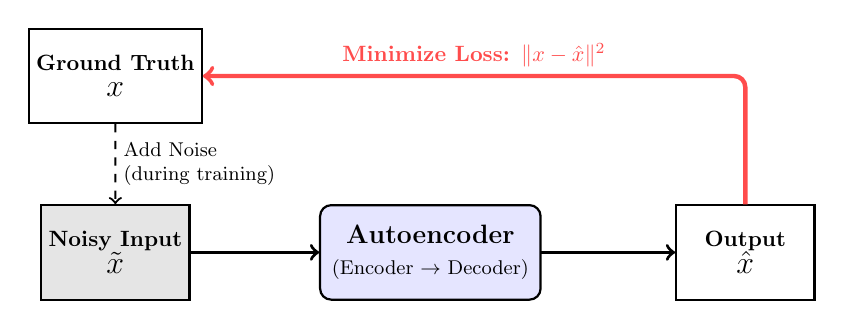
\begin{tikzpicture}[scale=0.8, transform shape]
    % --- Nodes ---
    
    % 1. Ground Truth (Top Left)
    \node[draw, thick, fill=white, minimum width=2.2cm, minimum height=1.5cm, align=center] (clean) at (0, 2.8) {
        \textbf{Ground Truth}\\
        \Large $x$
    };
    
    % 2. Noisy Input (Bottom Left)
    \node[draw, thick, fill=gray!20, minimum width=2.2cm, minimum height=1.5cm, align=center] (noisy) at (0, 0) {
        \textbf{Noisy Input}\\
        \Large $\tilde{x}$
    };
    
    % 3. Autoencoder (Center)
    \node[draw, thick, fill=blue!10, rounded corners, minimum width=3.5cm, minimum height=1.5cm, align=center, font=\large] (ae) at (5, 0) {
        \textbf{Autoencoder}\\
        \small (Encoder $\to$ Decoder)
    };
    
    % 4. Output (Bottom Right)
    \node[draw, thick, fill=white, minimum width=2.2cm, minimum height=1.5cm, align=center] (output) at (10, 0) {
        \textbf{Output}\\
        \Large $\hat{x}$
    };
    
    % --- Arrows ---
    
    % Noise Process (Down)
    \draw[->, thick, dashed] (clean) -- node[midway, right, font=\small, align=left] {Add Noise\\(during training)} (noisy);
    
    % Forward Pass (Right)
    \draw[->, very thick] (noisy) -- (ae);
    \draw[->, very thick] (ae) -- (output);
    
    % Loss Calculation (Up and Left)
    % Connecting Output back to Ground Truth for loss
    \draw[->, red!70, ultra thick, rounded corners] (output.north) -- (10, 2.8) -- node[midway, above, font=\bfseries] {Minimize Loss: $\|x - \hat{x}\|^2$} (clean.east);

\end{tikzpicture}

    \begin{tcolorbox}[colback=yellow!10, colframe=orange!50, title=\textbf{How it works}]
    \begin{itemize}
        \item Take clean image $x$.
        \item Corrupt it to get $\tilde{x}$.
        \item Force AE to map $\tilde{x} \rightarrow x$.
    \end{itemize}
    \end{tcolorbox}


\end{frame}

% --- SLIDE: Application - Anomaly Detection ---
\begin{frame}{Application 4: Anomaly Detection}

\textbf{Concept:} The network learns to reconstruct "Normal" data perfectly. When it sees an anomaly, it fails to reconstruct it.

\vspace{0.5em}
\centering
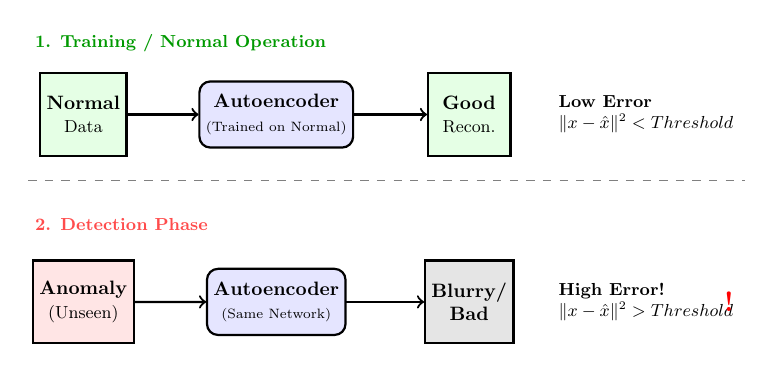
\begin{tikzpicture}[scale=0.7, transform shape]

    % --- SCENARIO 1: NORMAL (Top) ---
    \node[anchor=west, font=\bfseries\small, green!60!black] at (-3, 2.5) {1. Training / Normal Operation};
    
    % Input Normal
    \node[draw, thick, fill=green!10, minimum width=1.5cm, minimum height=1.5cm, align=center] (norm_in) at (-2, 1.2) {
        \textbf{Normal}\\
        \small Data
    };

    % Autoencoder (Shared)
    \node[draw, thick, fill=blue!10, rounded corners, minimum width=2.5cm, minimum height=1.2cm, align=center] (ae_top) at (1.5, 1.2) {
        \textbf{Autoencoder}\\
        \scriptsize (Trained on Normal)
    };

    % Output Normal
    \node[draw, thick, fill=green!10, minimum width=1.5cm, minimum height=1.5cm, align=center] (norm_out) at (5, 1.2) {
        \textbf{Good}\\
        \small Recon.
    };

    % Result
    \node[right, align=left, font=\small] at (6.5, 1.2) {
        \textbf{Low Error}\\
        $\|x - \hat{x}\|^2 < \text{Threshold}$
    };
    \node[right, green!60!black, font=\Large] at (9.5, 1.2) {\checkmark};

    % Arrows
    \draw[->, thick] (norm_in) -- (ae_top);
    \draw[->, thick] (ae_top) -- (norm_out);


    % --- SEPARATOR LINE ---
    \draw[dashed, gray] (-3, 0) -- (10, 0);


    % --- SCENARIO 2: ANOMALY (Bottom) ---
    \node[anchor=west, font=\bfseries\small, red!70] at (-3, -0.8) {2. Detection Phase};

    % Input Anomaly
    \node[draw, thick, fill=red!10, minimum width=1.5cm, minimum height=1.5cm, align=center] (anom_in) at (-2, -2.2) {
        \textbf{Anomaly}\\
        \small (Unseen)
    };

    % Autoencoder (Same one)
    \node[draw, thick, fill=blue!10, rounded corners, minimum width=2.5cm, minimum height=1.2cm, align=center] (ae_bot) at (1.5, -2.2) {
        \textbf{Autoencoder}\\
        \scriptsize (Same Network)
    };

    % Output Poor
    \node[draw, thick, fill=gray!20, minimum width=1.5cm, minimum height=1.5cm, align=center] (anom_out) at (5, -2.2) {
        \textbf{Blurry/}\\
        \textbf{Bad}
    };

    % Result
    \node[right, align=left, font=\small] at (6.5, -2.2) {
        \textbf{High Error!}\\
        $\|x - \hat{x}\|^2 > \text{Threshold}$
    };
    \node[right, red, font=\Large] at (9.5, -2.2) {\textbf{!}};

    % Arrows
    \draw[->, thick] (anom_in) -- (ae_bot);
    \draw[->, thick] (ae_bot) -- (anom_out);

\end{tikzpicture}

% \vspace{0.8em}
\begin{tcolorbox}[colback=yellow!10, colframe=orange!50, title=\textbf{Real-World Use Cases}]
\begin{itemize}
    \item \textbf{Credit Card Fraud:} Normal transactions reconstruct well, theft looks weird.
    \item \textbf{Manufacturing:} Detect defective parts on an assembly line.
\end{itemize}
\end{tcolorbox}

\end{frame}


% --- PART 6: SUMMARY ---
\section{References}


\begin{frame}{References}
    \begin{itemize}
        \item Aurélien Géron, \textit{Hands-On Machine Learning with Scikit-Learn, Keras, and TensorFlow}
        \item Andrew Ng, \textit{Machine Learning Specialization} (Coursera/DeepLearning.AI)
    \end{itemize}

    \vspace{2em}
    
    \begin{flushleft}
        \small\textit{Slides contributed by Mohamed Eltayeb}
    \end{flushleft}
    
\end{frame}
